%% Template para disserta????o/tese na classe UFBAthesis
%% versao 1.0
%% (c) 2005 Paulo G. S. Fonseca
%% (c) 2012 Antonio Terceiro
%% (c) 2014 Christina von Flach
%% www.dcc.ufba.br/~flach/ufbathesis

%% Carrega a classe ufbathesis
%% Opcoes: * Idiomas
%%           pt   - portugues (padrao)
%%           en   - ingles
%%         * Tipo do Texto
%%           bsc  - para monografias de graduacao
%%           msc  - para dissertacoes de mestrado (padrao)
%%           qual - exame de qualificacao de mestrado
%%           prop - exame de qualificacao de doutorado
%%           phd  - para teses de doutorado
%%         * M??dia
%%           scr  - para vers??o eletr??nica (PDF) / consulte o guia do usuario
%%         * Estilo
%%           classic - estilo original a la TAOCP (deprecated)
%%           std     - novo estilo a la CUP (padrao)
%%         * Paginacao
%%           oneside - para impressao em face unica
%%           twoside - para impressao em frente e verso (padrao)
\documentclass[bsc, classic, a4paper]{ufbathesis}
\usepackage[utf8]{inputenc}
\usepackage{indentfirst}
\usepackage{booktabs}
\usepackage{float}

\makeatletter  
\def\NAT@parse{\typeout{This is a fake Natbib command to fool Hyperref.}}  
\makeatother  

\usepackage{hyperref}
\usepackage{graphicx}

%% Preambulo:
%% coloque aqui o seu preambulo LaTeX, i.e., declara????o de pacotes,
%% (re)definicoes de macros, medidas, etc.

%% Identificacao:

% Universidade
\university{UNIVERSIDADE FEDERAL DA BAHIA}

% Endereco (cidade)
% e.g. \address{Campinas}
\address{Salvador}

% Instituto ou Centro Academico
% e.g. \institute{Centro de Ciencias Exatas e da Natureza}
% Comente se nao se aplicar
\institute{Departamento de Engenharia Elétrica e Computação}

% Nome da biblioteca - usado na ficha catalografica
% default: nome da biblioteca do Instituto de Matematica
\library{BIBLIOTECA REITOR MACÊDO COSTA}

% Programa de pos-graduacao
% e.g. \program{Pos-graduacao em Ciencia da Computacao}
\program{Departamento de Engenharia Elétrica e de Computação}

% ?rea de titulacao
\majorfield{Engenharia de Computação}

% Titulo da dissertacao/tese
% e.g. \title{Sobre a conjectura $P=NP$}
\title{Análise do tempo da latência de interrupção no Raspberry Pi em diferentes patches de tempo real para o kernel Linux}

% Data da defesa
% e.g. \date{19 de fevereiro de 2003}
\date{DIA de MÊS de ANO}

% Autor
% e.g. \author{Jose da Silva}
\author{Taian Fonseca Feitosa}

% Orientador(a)
% Opcao: [f] - para orientador do sexo feminino
% e.g. \adviser[f]{Profa. Dra. Maria Santos}
\adviser{Paul Regnier}

% Orientador(a)
% Opcao: [f] - para orientador do sexo feminino
% e.g. \coadviser{Prof. Dr. Pedro Pedreira}
% Comente se nao se aplicar
% \coadviser{NOME DO(DA) CO-ORIENTADOR(A)}

%% Inicio do documento
\begin{document}

\pgcompfrontpage{}

%%
%% Parte pre-textual
%%
\frontmatter

%\pgcomppresentationpage
% Se seu trabalho for uma disserta??o de mestrado do PGCOMP, use a linha acima
%\presentationpage
% Se for qualificacao, use \presentationpage

% Ficha catalogrofica
\authorcitationname{Feitosa, Taian Fonseca} % e.g. Terceiro, Antonio Soares de Azevedo
\advisercitationname{Regnier, Paul} % e.g. Chavez, Christina von Flach Garcia
%\coadvisercitationname{NOME DO SEU CO-ORIENTADOR EM CITACOES} % e.g. Mendonca, Manoel Gomes de
\catalogtype{Trabalho de Conclusão de Curso} % e.g. ``Tese (doutorado)''
\catalogtopics{1. Raspberry Pi. 2. Sistemas de tempo real. 3. PREEMPT-RT. 4. Drones. 5. Sistemas embarcados} % e.g. ``1. Complexidade Estrutural. 2. Engenharia de Software''
\catalogcdd{CDD 20.ed. XXX.YY} % e.g. ``CDD 20.ed. XXX.YY'' (esse n??mero vai lhe ser dado pela biblioteca)
\catalogingsheet

% Termo de aprovacaoo
% Se seu trabalho for Tese de Doutorado, inclua comitteemember 4 e 5
\approvalsheet{Salvador, DIA de MES de ANO}{
  \comittemember{Profa. Dra. Professora 1}{Universidade XYZ}
  \comittemember{Prof. Dr. Professor 2}{Universidade 123}
  \comittemember{Profa. Dra. Professora 3}{Universidade ABC}
%  \comittemember{Prof. Dr. Professor 4}{Universidade HJKL}
%  \comittemember{Profa. Dra. Professora 5}{Universidade QWERTY}
}

% Dedicatoria
% Comente para ocultar
\begin{dedicatory}
Dedicatória
\end{dedicatory}

% Agradecimentos
% Se preferir, crie um arquivo ?? parte e o inclua via \include{}
\acknowledgements
Agradecimentos

% Epigrafe
% Comente para ocultar
% e.g.
\begin{epigraph}[Um dia]{Eu mesmo}
Epígrafe
\end{epigraph}

% Resumo em Portugues
% Se preferir, crie um arquivo separado e o inclua via \include{}
\begin{resumo}
  Este trabalho apresenta um protocolo que torna o uso compartilhado de
  Ethernet eficiente para dar suporte aos sistemas de tempo real
  modernos.  O protocolo foi especificado formalmente e sua corre��o
  foi atestada automaticamente atrav�s de um verificador de modelo. Em
  seguida, um prot�tipo foi realizado numa plataforma operacional
  de tempo real.  Os resultados experimentais confirmaram a capacidade
  do protocolo em atender os objetivos definidos na sua proposta.

  As aplica��es que podem se beneficiar deste protocolo s�o
  principalmente aquelas compostas de dispositivos heterog�neos e
  distribu�dos que t�m restri��es temporais de natureza cr�ticas e
  n�o-cr�ticas.  Utilizando o protocolo proposto, tais sistemas podem
  utilizar o mesmo barramento Ethernet de forma eficiente e
  previs�vel. A utiliza��o do barramento � otimizada atrav�s da
  aloca��o apropriada da banda dispon�vel para os dois tipos de
  comunica��o. Al�m disso, o protocolo, compat�vel com os dispositivos
  Ethernet comuns, define um controle descentralizado do acesso ao
  meio que garante flexibilidade e confiabilidade � comunica��o.

  

    \begin{keywords}
     Ethernet, Tempo Real, Toler�ncia a falhas, Especifica��o Formal. 
    \end{keywords}
\end{resumo}



% Resumo em Ingles
% Se preferir, crie um arquivo separado e o inclua via \include{}
\abstract
Modern computer systems are capable of performing many tasks and also need to meet a variety of requirements. Some systems have time requirements and need to respond quickly and correctly to external events such as cars, aircraft, robotic systems, and other mechatronic systems, where a delayed response may compromise system integrity. For this, specific operating systems are designed to meet these requirements, the real-time operating systems. These external events are signaled to the processor through the interrupt mechanism. To keep the system responsive, these interrupts need to be addressed in a short and predictable time. As systems are increasingly complex, accurate analysis models do not exist, so measurement strategies are the best way to verify system responsiveness. One of the most popular embedded systems is the Raspberry Pi, a small, low-cost, low-power platform that uses Linux, one of the most popular operating systems in the world. This makes Raspberry Pi one of the most widely used platforms for the development of embedded systems in various projects. This work analyzes Raspberry's latency when responding to external events on standard Linux and Preempt-RT, a realtime patch for Linux.

% Palavras-chave do resumo em Ingles
\begin{keywords}
Raspberry Pi; Real-time systems; Preempt-RT; Embedded systems
\end{keywords}


% Sumario
% Comente para ocultar
\tableofcontents

% Lista de figuras
% Comente para ocultar
\listoffigures

% Lista de tabelas
% Comente para ocultar
\listoftables

%%
%% Parte textual
%%
\mainmatter

% Eh aconselhavel criar cada capitulo em um arquivo separado, digamos
% "capitulo1.tex", "capitulo2.tex", ... "capituloN.tex" e depois
% inclui-los com:
\xchapter{Introdução}{}

 % A história dos drones pode parecer recente diante dos avanços tecnológicos que baratearam as tecnologias envolvidas nos modelos mais conhecidos, mas, ao buscar sua origem, percebemos que estamos usando drones há mais de um século. No livro \textit{The Future of Drone Use: Opportunities and Threats from Ethical and Legal Perspectives} \cite{Custers2016}, considera-se que o primeiro uso de um drone registrado ocorreu em julho de 1849, quando as forças austríacas tentaram lançar balões incendiários com explosivos e uma bomba relógio para fazer os mesmo caírem sobre a cidade de Veneza. O drone como é conhecido hoje foi concebido por Abe Karem em 1977, quando criou um drone que era controlado por 3 pessoas, em vez de 30, como exigido pelos drones da época \cite{Buzzo2015}.

% \section{Apresentação}

Sistemas computacionais modernos possuem cada vez mais requisitos e complexidade para atender o seu crescente número de aplicações. Alguns sistemas possuem requisitos temporais, estes são chamados de sistemas de tempo real. Um Sistema de Tempo Real (STR) tem que garantir que a resposta, além de correta, será entregue a tempo, de modo a garantir que este sistema seja previsível e possa ter garantias temporais. Sistemas embarcados como carros e aeronaves, plantas industriais e sistemas robóticos, são apenas alguns exemplos de sistemas que precisam de uma resposta correta e em tempo restrito para que a aplicação funcione corretamente.

Para termos um Sistema de Tempo Real, é necessário que o sistema operacional esteja preparado para lidar com esse tipo de aplicação específica, pois, com a evolução tecnológica do hardware, surgem novos fatores que podem trazer variações no tempo de resposta do sistema. Por exemplo, temos os adventos de memória cache, acesso direto à memória, co-processamento, predição de instruções, unidades multicore, pipelines e execução fora de ordem, que constituem fontes de indeterminismo \cite{Liu2000, Pratt2004}. Todos esses fatores são desafios a serem resolvidos para permitir que Sistema Operacional de Propósito Geral possa dar garantias temporais similares a um Sistema Operacional de Tempo Real (SOTR) dedicado.

\section{Motivação}

Hoje, os drones são muito populares, tanto para uso recreativo quanto para diversos outros fins. O Departamento de Controle do Espaço Aéreo Brasileiro através da Instrução de Comando da Força Aérea (ICA) 100-40 \cite{CEA2018} define os modelos usados apenas para fins recreativos como \textit{aeromodelos} e os outros modelos como \textit{Aeronaves Remotamente Pilotada - ARP}. Normalmente, os \textit{aeromodelos} são operados por humanos através de um controle remoto, enquanto as \textit{ARP} também podem ser automáticos ou autônomos. As \textit{ARPs} automáticas são modelos capazes de operar por conta própria e também podem ser controlados manualmente a qualquer momento, enquanto os autônomos têm seu caminho definido anteriormente e não podem ter intervenção humana durante a realização da missão.

Para que o drone possa executar uma missão automática ou autonomamente, é necessário um sistema de controle capaz de interpretar os dados dos sensores, fazer cálculos e tomar decisões. Alguns modelos de drones possuem sistemas operacionais e sensores embarcados que são suficientes para que se projete uma missão automática. Em outros casos, como o modelo \textit{Parrot AR.Drone 2.0} \cite{Parrot2019a}, utilizado pelo LaSid, o sistema é muito simples para ser capaz de realizar tarefas mais complexas. Uma solução é adotar um sistema auxiliar acoplado ao drone, capaz de interagir com as APIs do sistema do drone. Um sistema que se adapta bem a essa tarefa é o Raspberry Pi.

O Raspberry Pi é um computador do tamanho de um cartão de crédito que pode se conectar a uma TV ou monitor e usar periféricos como mouse e teclado \cite{RPF2019}. O sistema operacional padrão é o Linux, cuja distribuição principal é a Raspbian, com base na distribuição Debian. A possibilidade de usar o Linux torna o Raspberry Pi uma solução muito mais flexível em comparação com outras soluções de microcontroladores, como o Arduino, por exemplo.

A desvantagem vem do fato de que sistemas como o Arduino podem ser determinísticos, ou seja, sempre responder dentro de um tempo máximo calculado, enquanto o sistema Linux padrão não tem garantias temporais para responder a um evento externo. No entanto a frequência de operação do processador do Raspberry Pi é muito superior à do Arduino (1200 MHz no modelo utilizado pelo LaSid contra 16 MHz do Arduino Uno, modelo mais comum), e portanto, uma solução baseada no Raspberry Pi quase sempre pode responder mais rápido do que uma solução semelhante baseada no Arduino.

Na maioria das aplicações, o comportamento do Raspberry Pi pode ser satisfatório. Em aplicações críticas, no entanto, uma única resposta atrasada pode significar uma falha catastrófica. Para lidar com esses cenários em que o tempo máximo de resposta deve ser previsível, foram criados patches para o kernel Linux a fim de torná-lo um Sistema Operacional de Tempo Real. 

Durante a realização deste trabalho, não foi encontrado nenhum trabalho que verifique o determinismo do Raspberry Pi levando em conta os diferentes tipos de implementação do sistema operacional Linux e o impacto das interrupções nas garantias temporais. As análises da latência de interrupção costumam ser testes de caixa preta: testes onde o funcionamento interno é desconhecido, sendo medido apenas o tempo entre o sistema receber um estímulo externo que requer a atenção do sistema e o mesmo responder a esse estímulo com uma resposta visível; em contraste com testes de caixa branca: testes onde é analisado o funcionamento interno do objeto sendo medido. Ao fazer uma análise em mais baixo nível, isto é, levando em conta os mecanismos de interrupção presentes no kernel e o comportamento diferente deles, é possível separar o tempo de resposta do sistema do tempo de resposta da aplicação.

\section{Objetivos}

\subsection{Objetivo principal}

O objetivo deste trabalho é verificar o determinismo da plataforma Raspberry Pi 3 Model B dotado do sistema operacional Linux padrão, Linux Preempt-RT e Linux com o Xenomai em diferentes cenários de execução de aplicações com requisitos temporais. Para este feito, realiza-se experimentos para quantificar as diversas latências do sistema em vários cenários de execução, de forma a ajudar no desenvolvimento de aplicações com requisitos temporais nesta plataforma. Para realizar os experimentos foi o usado o módulo INTSight, que é um módulo kernel para realizar benchmarks das latências dos diferentes mecanismos de interrupção desenvolvido por Luis Gerhorst \cite{Gerhorst2018}, que será apresentado na seção \ref{INTSight}. Espera-se que esses experimentos ajudem na decisão do tipo de plataforma e de sistema a ser utilizado de acordo com os requisitos da aplicação desejada.

\subsection{Objetivos intermediários}

O objetivo principal se desdobrou nos seguintes objetivos intermediários:

\begin{itemize}
    \item Adaptar o INTSight para o Raspberry Pi;
    \item Adaptar o INTSight no kernel padrão do Linux e realizar as medições;
    \item Adaptar o INTSight no patch Preempt-RT e realizar as medições;
    \item Adaptar o INTSight no patch Xenomai e realizar as medições;
    \item Analisar o resultado obtido nas medições;
\end{itemize}

Destes objetivos intermediários, a adaptação do Xenomai não foi cumprida por este trabalho. As dificuldades estão relatadas na seção \ref{Dificuldades}.

\section{Organização}

No capítulo \ref{cap2} irei apresentar alguns trabalhos relacionados e quais as estratégias utilizadas pelos autores em cada um para realizar suas medições ou análises. A descrição dos modelos de SO utilizados nas medições além de características do Raspberry Pi Model B serão apresentadas no capítulo \ref{cap3}. A apresentação e análise de resultados experimentais está no capítulo \ref{cap4}, onde faço uma comparação entre os modelos de interrupção e os SO's. Na última parte, no capítulo \ref{cap5}, serão apresentadas as dificuldades encontradas durante a realização deste trabalho e ideias para continuação do trabalho no futuro.

\xchapter{Revisão bibliográfica}{Base teórica}

O que outras pessoas fizeram sobre esse tema.

\section{Quem fez o quê}

Paul, testes \cite{Regnier2008}

Interrupt response times on Arduino and Raspberry Pi \cite{Solc2016}

INTSight \cite{Gerhorst2018}

Mais...

\section{Como fizeram}
\section{Mais algo?}
\xchapter{Especificação do problema e a solução proposta}{Opcional}

Detalhes do trabalho a resolver.

Outro parágrafo.

\section{Sistemas de tempo real}
\section{Raspberry}

\chapter{Experimentos}
\label{cap:experimentos}

\section{Introdu��o}
\label{sec:introImp}

Neste cap�tulo, apresentar-se-� um estudo comparativo das quatro plataformas
apresentados no cap�tulo \ref{capSOTR}. Os experimentos realizados n�o tem
por objetivo de ser exaustivos. Eles apenas foram utilizados para entender
o comportamento temporal dos diferentes sistemas, tendo como foco principal
as lat�ncias de interrup��o e as lat�ncias de escalonamento relacionadas 
a camada de rede.

bla bla bla...


\section{Medidas de lat�ncias}
\label{sec:medLat}

Na se��o \ref{sec:latIRQ} do cap�tulo \ref{cap:SOTR}, o problema da medida das
lat�ncias de interrup��o foi brevemente apresentado. Uma das dificuldade apontada
foi esta da medi��o do instante exata no qual uma determinada interrup��o acontece
num certo hardware. Tendo como objetivo a compara��o das plataformas Linux, Linux
PREEMPT-RT, RTAI e Xenomai, adotou-se uma metodologia experimental simples,
inspirada de \cite{Proctor01}, que apesar de ser quase exclusivamente baseada nos
recursos internos do computador, permitiu obter resultados qualitativos bastante
significativos.

\subsection{O dispositivo experimental}
\label{sec:dispExp}

O dispositivo experimental utilizou a porta paralela, conectando um dos pinos
habilitados para escrita, presentemente o pino 9, ao pino 10 de interrup��o.  A
descri��o desta manipula��o e de v�rios exemplos de m�dulos para escrever na porta
paralela e capturar as interrup��es desta mesma porta foram encontrados no excelente
livro \ing{Linux Device Drivers} \cite{Corbet05}.  Para acessar valores de tempo
numa precis�o da ordem do $\mu s$, utilizou-se o contador do processador chamado de
\ing{Time Stamp Counter} (TSC). Para realizar as medidas, um m�dulo $M$ especifico
foi desenvolvido para oferecer fun��es de \cod{ioctl} que implementam as seguintes
opera��es:

\begin{itemize}
\item Acessar os 64 bits do TSC e gravar o valor na mem�ria.
\item Escrever na porta de entrada e sa�da 0x378 da porta paralela para gerar
  interrup��es de hardware.
\item Requisitar a captura das interrup��es na linha 7 associada a porta paralela e
  registrar o tratador associado que executa a �nica opera��o de gravar o TSC.
\item Implementar um canal de comunica��o FIFO  ass�ncrono para transferir os dados
  coletados em modo protegido para o espa�o usu�rio.
\end{itemize}

Este conjunto de fun��es de \cod{ioctl} � exportado para os processos executando em
modo usu�rio atrav�s de um arquivo especial \cod{/dev/M} do sistema de arquivo. 

As medidas foram realizadas acompanhando o seguinte roteiro.  Ap�s a inser��o do
m�dulo $M$ no \kernel, um processo $P$, executando em modo usu�rio, abre o arquivo
especial \ing{/dev/M} para poder acessar as fun��es \ing{ioctl} disponibilizadas
pelo m�dulo $M$. No instante $t_1$ no qual $P$ executa o \cod{ioctl} de escrita no
pino 9 da porta paralela, o valor do TSC � memorizado na mem�ria do \kernel. Alguns
micro-segundos depois, o tratador de interrup��o � executado pelo \kernell e o valor
do TSC � gravado novamente no instante $t_2$. A lat�ncia de interrup��o $t_2 - t_1$
� ent�o deduzida e armazenada numa mem�ria tamp�o lida periodicamente pelo processo
$P$. 

Este m�todo experimental tem as seguintes limita��es. Quando uma interrup��o
acontece, o estado do processador � sempre o mesmo, ou seja, antes de um
interrup��o, o processador est� sempre executando o processo usu�rio $P$ que acessa
a fun��o de \cod{ioctl} do m�dulo $M$ para escrever na porta paralela.  Portanto, a
presen�a de outros processos usu�rios sobrecarregando o processador n�o pode
interferir nas medidas. Uma outra limita��o provem do tempo de lat�ncia da pr�pria
porta paralela, que leva um certo tempo para estabilizar sua sa�da, na hora da
escrita. No entanto, os resultados obtidos usando esta metodologia podem servir para
medir um valor m�nimo do tempo de lat�ncia e para comparar diferentes plataformas
operacionais. Al�m disso, o impacto causado pela presen�a de outras atividades gerando
interrup��es pode ser observado. No caso deste trabalho, a placa de rede foi utilizado
para este efeito.

Observa que para evitar qualquer interfer�ncia nas medidas de lat�ncia, no caso do
Linux e de \preempt, o conjunto dos valores mensuradas foi salvo na mem�ria e
somente transferido para o sistema de arquivo depois do fim da execu��o do
experimento. Para as plataformas RTAI e Xenomai, foram utilizados os canais
\cod{RT-FIFO} de tempo real oferecidos pela API de ambas plataformas. A
implementa��o, sem \ing{lock}, destes canais garante a princ�pio a aus�ncia de
interfer�ncia com a execu��o das tarefas de tempo real no sistema.
 
No caso das duas plataformas RTAI e Xenomai, medidas complementares da lat�ncia de
escalonamento foram realizadas para avaliar a capacidade destas plataformas em
executar opera��es de transmiss�o de mensagens Ethernet com garantias
temporais. Para este efeito, o m�dulo $M$ foi acrescentado da seguinte maneira. Na
sua inser��o, ele cria uma tarefa $T$ (\ing{thread} de \kernel) que � acordada pelo
tratador de interrup��o da porta paralela. Quando a tarefa $T$ acorda, ela grava o
valor $t_3$ do TSC. Em seguida, $T$ executa a transmiss�o de um pacote Ethernet de
64 bytes, utilizando a fun��o \hardStartXmit, disponibilizada pelo controlador da
placa de rede.  No instante no qual esta fun��o � chamada, $T$ grava o valor $t_4$
do TSC. O valor da diferencia $t_3 - t_2$ representa portanto a lat�ncia de
escalonamento da tarefa $T$ e o valor $t_4 - t_3$, o tempo de execu��o necess�rio
para transmitir um pacote na rede.


\subsection{Modo operacional}
\label{sec:modOp}

Para realizar as medidas de lat�ncia de interrup��o e de tratamento, o processo $P$
executou escritas no pino 9 da porta paralela com uma freq��ncia aproximada de $20
Hz$. J� que as medidas n�o dependem do valor do instante inicial da escrita, esta
freq��ncia foi obtida utilizando uma chamada a fun��o \cod{sleep} com um argumento
de $50 ms$.  Esta freq��ncia relativamente baixa foi escolhida para garantir o
processamento completo de todas as opera��es de medida e o escalonamento eventual de
outros processos entre cada escrita na porta paralela.  No entanto, resultados
quantitativamente id�nticos ser�o mostrados na se��o \ref{} para o RTAI e o Xenomai
com uma freq��ncia de $1000 Hz$.

No caso destas duas plataformas, RTAI e do Xenomai, o foco foi dado a lat�ncia de
interrup��o associadas ao dom�nio prim�rio, descrito na se��o \ref{sec:adeos}, j�
que a proposta do protocolo \doriss � oferecer garantias temporais para tarefas de
tempo real cr�ticas.

Cada um dos cen�rios de medida durou aproximadamente 70 segundos e foi realizados
usando um ambiente gr�fico. No entanto, experimentos em modo \ing{single}, no qual o
n�mero de \ing{thread} de \kernell � m�nimo, deram os mesmos resultados
quantitativos. Nos primeiros 10 segundos dos experimentos, o processo $P$ gerou as
interrup��es na freq��ncia de $20 Hz$ sem que nenhum outra atividade interfere.

Entre a d�cima e a vig�sima segunda, um estresse de comunica��o foi aplicado ao
sistema via a rede Ethernet durante aproximadamente 10 segundos. O estresse aplicado
utilizou o comando \cod{ssh} da seguinte maneira. Uma m�quina remota executou o
comando \ing{shell} \cod{ssh IP "echo \$ITER >> /tmp/stress"}, 60 vezes
consecutivas.  Nesta express�o, $IP$ era o n�mero IP da esta��o na qual as medidas
eram realizadas e $\$ITER$ era o �ndice de itera��o do la�o de execu��o do
comando. Constatou-se que 60 vezes corespondiam aproximadamente a um tempo de
execu��o de 10 segundos.

A escolha deste tipo de estresse se justificou por duas raz�es principais.  Em
primeiro lugar, a placa de rede utiliza a linha de interrup��o 18 cuja prioridade �
menor que a prioridade da porta paralela. Portanto, as interrup��es geradas nesta
pela placa de rede n�o deveriam interferir a princ�pios nas medidas efetuadas.  Em
segundo lugar, j� que este trabalho tem por objetivo a implementa��o de um protocolo
de rede baseado em Ethernet, pude-se avaliar a capacidade das diferentes plataformas
em garantir uma lat�ncia determin�stica no tratamento das interrup��es, mesmo na
presen�a de um estresse de comunica��o.

Todos os experimentos foram realizados pelo menos tr�s vezes e selecionou-se
os cen�rios com as lat�ncias maiores no pior caso.

% Este estresse foi criado simplesmente, utilizando uma comunica��o UDP do tipo
% cliente-servidor. Para gerar as interrup��es no computador no qual as medidas eram
% efetuadas, confi\-gurou-se este como servidor da comunica��o UDP. O processo servidor
% foi criado utilizando a API das bibliotecas \cod{pthread} com a prioridade mais
% alta poss�vel. O cliente, instalado numa m�quina remota, foi configurado para 
% transmitir pequenos pacotes de 64 \ing{bytes} na freq��ncia m�xima permitida pela
% rede, ou seja, com uma freq��ncia de quase $200 kHz$ (um pacote a cada $5 \mu s$).
% Desta forma, 200.000 interrup��es por segundos aconteciam na placa de rede
% do servidor.

\subsection{Resultados experimentais}
\label{sec:resulExp}

O dispositivo experimental descrito nas se��es \ref{sec:dispExp} e \ref{sec:modOp}
foi implementado em computadores Pentium 4 com processadores de 2.4 Ghz e 512 Mb de
mem�ria. Os resultados experimentais s�o apresentados pelo meio de figuras nas quais
o eixo horizontal representa o tempo variando de 0 a 70 segundos e o eixo vertical
representa a lat�ncia de interrup��o em $\mu s$ medida a cada escrita na porta
paralela. 

As seguintes configura��es das quatro plataformas Linux, PREEMP-RT, RTAI e Xenomai
foram utilizadas. A vers�o do \kernell de Linux 2.6.19.7 foi utilizada para os
testes do \kernell Linux, de RTAI e de Xenomai \cite{kernel}. Nos tr�s casos,
compilou-se o \kernell Linux com a configura��o de preemp��o habilitada
(\ing{Low-Latency}). Apesar de existir vers�es do \kernell mais recentes suportadas
por estas tr�s plataformas, RTAI e Xenomai disponibilizavam \ing{patchs} est�veis
para esta vers�o do \kernell no in�cio deste trabalho, em janeiro de 2007. J� que
estas duas plataformas s�o baseados no Adeos, como foi visto na descri��o da se��o
\ref{sec:adeos}, suas propriedades temporais n�o dependem, a princ�pio, do \kernel
Linux. Considerou-se ent�o desnecess�rio atualizar a vers�o do \kernell. No entanto,
utilizou-se as vers�es mais recentes das duas distribui��es do RTAI e Xenomai. No
caso do RTAI, a vers�o \ing{magma} foi baixada diretamente do site \cite{RTAI},
utilizando o sistema de controle de vers�o \ing{CVS}. Para o Xenomai, utilizou-se a
vers�o 2.4-rc5 dispon�vel desde outubro 2007 \cite{Xenomai}.

Para estas duas plataformas, os diferentes testes de lat�ncias fornecidos foram
utilizados, dando resultados de menos de $10 \mu s$ no pior caso para a lat�ncia de
interrup��o, conforme os padr�es da arquitetura Intel Pentium 4. Observa-se que, em
ambas plataformas, desabilitou-se as interrup��es de gerenciamento do sistema
(\ing{SMI}), conforme as recomenda��es dos desenvolvedores \cite{RTAI,
  Xenomai}. Isto permitiu cancelar uma lat�ncia da ordem de $2.5ms$ que aparecia nos
testes periodicamente a cada 32 segundos. No caso do Linux e de PREEMP-RT, as
interrup��es de gerenciamento do sistema n�o foram desabilitadas. No entanto, n�o se
observou nenhuma lat�ncia da ordem de $2.5ms$ nos experimentos relativos a estas duas
plataformas. Provavelmente, porque a interrup��o peri�dica de SMI aconteceu num
intervalo de tempo sem medida.

Em rela��o ao \ing{patch} PREEMPT-RT, ele tem evolu�do rapidamente no decorrer do
seus dois anos de vida. Notadamente, desde a vers�o 2.6.21, o \kernell Linux
disponibiliza temporizadores de alta precis�o para as arquiteturas x86, ARM e PPC, o
que permite ao \ing{patch} \preemptt de trabalhar com resolu��o da ordem do $\mu s$
(ver se��o \ref{sec:preemptRT}) no escalonamento de tarefas. Portanto, utilizou-se a
vers�o est�vel do \kernell em dezembro de 2007, isto �, a vers�o 2.6.23.9.

\subsubsection{Linux e \preempt}

\begin{figure}%
  \centering
  \subfloat[][Os tri�ngulos vermelhos correspondem aos piores casos.]{%
    \label{fig:klight1}%
    {\scalebox{1}{\input{fig/klight1}}}}\\
  \vspace{10pt}%
  \subfloat[][Os piores casos s�o representados no valor $15 \mu s$.]{%
    \label{fig:klight2}%
    {\scalebox{1}{\input{fig/klight2}}}}%
  \caption[Lat�ncia de interrup��o do Kernel Linux]{Lat�ncia de interrup��o do
    \kernell Linux 2.6.19.7, op��o \ing{Low-Latency}. As figuras
    \subref{fig:klight1} e \subref{fig:klight2} representam a mesma execu��o.  A
    freq��ncia de interrup��o de $20 Hz$ e os dois estresses (60 aberturas e
    fechamento de sess�o \cod{ssh}) s�o aplicados nos instantes 10s e 40s.  Na
    figura \subref{fig:klight2}, os piores casos s�o mostrados no valor $15 \mu s$ para
    deixar os detalhes das demais medidas aparecer.}
%    \subref{fig:ex3-d} describes the last sub-float.}%
  \label{fig:klight}%
\end{figure}

\begin{figure}%
  \centering
  \subfloat[Os tri�ngulos vermelhos correspondem aos piores casos.]{%
    \label{fig:preempt1}%
    {\scalebox{1}{\input{fig/preempt1}}}}\\
  \vspace{10pt}%
  \subfloat[][Os piores casos s�o representados no valor $15 \mu s$.]{%
    \label{fig:preempt2}%
    {\scalebox{1}{\input{fig/preempt2}}}}%
  \caption[Lat�ncia de interrup��o de \preemptt]{Lat�ncia de interrup��o do
    \kernell Linux 2.6.23.9, com o \ing{patch} \preemptt. As figuras
    \subref{fig:preempt1} e \subref{fig:preempt2} representam a mesma execu��o.  A
    freq��ncia de interrup��o de $20 Hz$ e os dois estresses (60 aberturas e
    fechamento de sess�o \cod{ssh}) s�o aplicados nos instantes 10s e 40s.  Na
    figura \subref{fig:preempt2}, os piores casos s�o mostrados no valor $15 \mu s$
    para deixar os detalhes das demais medidas aparecer.}
  \label{fig:preempt}%
\end{figure}

A figura \ref{fig:klight} apresenta as lat�ncias de interrup��o observadas para o
\kernell Linux padr�o. Durante os dois per�odos de $10 s$ nos quais o estresse
\cod{ssh} � aplicado, os piores casos de lat�ncia, representados pelos tri�ngulos
vermelhos na figura \ref{fig:klight1}, chegam quase a $10 ms$.  No detalhe da figura
\ref{fig:klight2}, na qual os piores casos s�o representados no valor arbitr�rio de
$15 \mu s$, percebe-se que na aus�ncia de estresse, os tempos de lat�ncias s�o
bastante est�veis, abaixo de $10 \mu s$, em acordo com valores encontrados na
literatura \cite{Proctor01, Rostedt07, Siro07}. Durante a aplica��o dos estresses, a
lat�ncia da maioria dos eventos aumenta apenas de $1 \mu s$. Alguns eventos isolados
chegam a atingir at� 13 $\mu s$ de lat�ncia, enquanto, nos piores casos, a lat�ncia
atingi quase 1000 vezes o caso m�dio sem estresse.

Resultados similares foram obtidos com \preemptt como pode ser observado
nas figuras \ref{fig:preempt1} e \ref{fig:preempt2}. Esta semelhan�a era
de se esperar, j� que o c�digo da camada de rede do Linux � bastante otimizado, e que,
conseq�entemente, as melhorias trazidas por \preemptt n�o afetam as caracter�sticas 
temporal desta camada.

No caso do Linux, $6$ eventos tiveram uma lat�ncia superior a $20 \mu s$ e no
\preemptt foram 11 eventos similares observados.  Portanto, apesar da maioria dos
eventos - mais de 400 ao total nos dois per�odos de estresse - n�o sofrer lat�ncia
superior a $14 \mu s$, pode-se concluir que a exist�ncia de lat�ncias de quase $10ms$
nos piores casos observados inviabilizam a utiliza��o destas duas plataformas no
contexto de sistema de tempo real cr�tico.


\subsubsection{RTAI e Xenomai}

Para os experimentos com RTAI e Xenomai, foi mencionado na se��o \ref{sec:dispExp}
que a transfer�ncia dos dados da mem�ria do \kernell para o sistema de arquivo foi
realizada com os canais \ing{RT-FIFO} proporcionados pela API destas duas
plataformas. Apesar das garantias ofertas pela implementa��o destas plataformas,
considerou-se a possibilidade que o acesso ass�ncrono aos canais \cod{RT-FIFO} por
um processo usu�rio poderia interferir nas medidas. Portanto, realizou-se os
experimentos com duas configura��es diferentes. Na primeira, os canais foram
consultados entre cada escrita na porta paralela e na segunda, o acesso s� aconteceu
a cada 20 escrita na porta paralela.  Em ambos os casos, a freq��ncia de escrita na
porta paralela era de $20 Hz$.

Os resultados destes dois modos de opera��o s�o apresentados nas figuras
\ref{fig:rtai} para RTAI e \ref{fig:xeno} para Xenomai. Constata-se que os eventos
extremos s�o mais raros e tem valores menores que no caso do Linux e do
\preempt. Com RTAI, observou-se um evento extremo de $165 \mu s$ na primeira
configura��o do experimento. Nos dois outros modos, um evento extremo isolado tamb�m
aconteceu, com a mesma ordem de grandeza.

Com o Xenomai, v�rios experimentos repetidos na primeira configura��o n�o permitiram
de observar evento extremo algum. No entanto, com o segundo modo experimental, no
qual a leitura do canal \cod{RT-FIFO} foi realizada com uma freq��ncia menor,
piores casos da mesma ordem de grandeza que no RTAI foram observados.

\begin{figure}%
  \centering
  \subfloat[O tri�ngulo vermelho corresponde a um pior caso isolado (de $165.3 \mu s$)]{%
    \label{fig:rtai2}%
    {\scalebox{1}{\input{fig/rtai2}}}}\\
  \vspace{10pt}%
  \subfloat[][M�dia sobre 20 eventos.]{%
    \label{fig:rtaiM2}%
    {\scalebox{1}{\input{fig/rtaiM2}}}}%
  \caption[Lat�ncia de interrup��o do RTAI]{Lat�ncia de interrup��o do \kernell
    Linux 2.6.19.7, com o \ing{patch} RTAI ``magma''. As figuras \subref{fig:rtai2}
    e \subref{fig:rtaiM2} representam execu��es na freq��ncia de interrup��o de $20
    Hz$. Os dois estresses (60 aberturas e fechamento de sess�o \cod{ssh}) s�o
    aplicados nos instantes 10s e 40s.  Na figura \subref{fig:rtai2}, o pior caso �
    mostrado no valor $15 \mu s$ para deixar os detalhes das demais medidas
    aparecer. Na figura \subref{fig:rtaiM2}, o canal RT-FIFO � consultado a cada 20
    interrup��es e a m�dia correspondente � calculada.}
  \label{fig:rtai}%
\end{figure}

\begin{figure}%
  \centering
  \subfloat[Valores instant�neos.]{%
    \label{fig:xeno1}%
    {\scalebox{1}{\input{fig/xeno1}}}}\\
  \vspace{10pt}%
  \subfloat[][M�dia sobre 20 eventos.]{%
    \label{fig:xenoM1}%
    {\scalebox{1}{\input{fig/xenoM1}}}}%
  \caption[Lat�ncia de interrup��o do Xenomai]{Lat�ncia de interrup��o do \kernell
    Linux 2.6.19.7, com o \ing{patch} Xenomai 2.4-rc5. As figuras \subref{fig:xeno1}
    e \subref{fig:xenoM1} representam execu��es na freq��ncia de interrup��o de $20
    Hz$. Os dois estresses (60 aberturas e fechamento de sess�o \cod{ssh}) s�o
    aplicados nos instantes 10s e 40s. Na figura \subref{fig:xenoM1}, o canal
    RT-FIFO � consultado a cada 20 interrup��es e a m�dia correspondente �
    calculada.}
  \label{fig:xeno}%
\end{figure}

Em conclus�o destes experimentos, considerou-se que as plataformas Linux e \preemptt
n�o podiam dar as garantias temporais necess�rias para a implementa��o do protocolo
\doris. Apesar de n�o constituir um conjunto suficiente de avalia��o, os resultados
com as plataformas RTAI e Xenomai mostraram que estas plataformas tem um
comportamento similares em que diz respeito a lat�ncia de interrup��o e que elas s�o
mais determin�sticas que Linux e \preempt. As ocorr�ncias de valores de lat�ncias
altas n�o ultrapassaram $200 \mu s$ e aconteceram numa freq��ncia m�xima 
de uma vez em 400 eventos. Do ponto de visto da implementa��o do protocolo 
\doris, estes resultados confirmaram o ganho significativo de se trabalhar com 
as plataformas RTAI e Xenomai. No entanto, a exist�ncia de piores casos 
demonstra a necessidade de utilizar mecanismo de toler�ncia para 
manter as garantias do protocolo de comunica��o, apesar destes eventos isolados.

Observa-se tamb�m que os experimentos foram realizadas numa
arquitetura especifica e que resultados quantitativamente diferentes teriam
provavelmente sido encontradas em outras configura��es de m�quinas. No entanto,
os resultados obtidos aqui s�o qualitativamente consistente com os resultados
apresentados em trabalhos similares \cite{McKenney05, Siro07, Dozio03}.

Al�m das medidas de interrup��o, medidas de lat�ncias de escalonamento e de tempos
de execu��o s�o mostradas nas figuras \ref{fig:latEscal}. Estas medidas foram
realizadas com a metodologia descrita na se��o \label{sec:dispExp}. A lat�ncia de
escalonamento corresponde ao tempo que passa entre a execu��o do tratador de
interrup��o e o instante no qual a tarefa $T$ suspensa come�a a executar. O tempo de
execu��o corresponde ao tempo do qual $T$ precisa para criar um pacote Ethernet de
64 bytes e transferi-lo para a placa de rede. Na aus�ncia de estresse, observa-se na
figura \ref{fig:latEscal} que estes tempos s�o est�vel em ambas plataformas. No caso
do RTAI, observa-se que a lat�ncia de escalonamento � da ordem de $1 \mu s$,
enquanto para Xenomai, ela � da ordem de $4 \mu s$.  Esta diferen�a se deve aos
modelos de tarefas diferentes nestas duas plataformas. Como foi visto na se��o
\ref{sec:adeos}, Xenomai privilegia a integra��o com o modo usu�rio do Linux e uma
das conseq��ncias deste modelo de desenvolvimento � a exist�ncia de uma sobrecarga
na troca de contexto de uma tarefa \cite{Gerum05}.

\begin{figure}%
  \centering
  \subfloat[Lat�ncias do RTAI]{%
    \label{fig:rtaiEsc}%
    {\scalebox{0.9}{\input{fig/rtaiEsc}}}}\\
  \vspace{20pt}
  \subfloat[Lat�ncias do Xenomai]{%
    \label{fig:xenoEsc}%
    {\scalebox{0.9}{\input{fig/xenoEsc}}}}\\
  \caption[Lat�ncia de interrup��o, de escalonamento e de execu��o do RTAI e do
  Xenomai]{Lat�ncia de interrup��o de escalonamento e de execu��o do Kernel Linux
    vers�o 2.6.19.7, com o \ing{patch} $RTAI$ e com o \ing{patch} Xenomai. As
    figuras \subref{fig:rtaiEsc} e \subref{fig:xenoEsc} apresentam as tr�s
    lat�ncias, na forma de histogramas sobreposto um em cima do outro.  A base
    coresponde a lat�ncia de interrup��o, a caixa do meio, a lat�ncia de
    escalonamento e a caixa de cima a lat�ncia de execu��o. Em ambos experimentos, a
    freq��ncia de interrup��o � $20 Hz$ e o canal RT-FIFO � consultado e as m�dias
    correspondentes calculadas a cada 20 eventos. Os dois estresses (60 aberturas e
    fechamento de sess�o \cod{ssh}) s�o aplicados nos instantes 10s e 40s.}
  \label{fig:latEscal}%
\end{figure}

Para observar o efeito do estresse sobre a lat�ncia de escalonamento e o tempo de
execu��o da tarefa $T$, a figura \ref{fig:stress} apresenta o detalhe das medidas
destes dois valores correspondendo aos experimentos das figuras
\ref{fig:rtai}\subref{fig:rtai2} e \ref{fig:xeno}\subref{fig:xeno1}.  Constata-se
que as duas plataformas comportam-se de forma bastante similares, com um aumento de
aproximadamente $4 \mu s$ na lat�ncia de interrup��o e de $2$ a $3 \mu s$ no tempo
de execu��o. O primeiro aumento corresponde provavelmente ao tratamento de uma (ou
duas nos piores casos) interrup��o da placa de rede, devida ao estresse. A segunda,
por ser mais espalhadas e ter valores menores, corresponde provavelmente a
atualiza��o da mem�ria tamp�o.

\begin{figure}%
  \centering
  \subfloat[][RTAI]{%
    \label{fig:rtaiStress}%
    {\scalebox{1}{% GNUPLOT: LaTeX picture with Postscript
\begingroup
  \makeatletter
  \providecommand\color[2][]{%
    \GenericError{(gnuplot) \space\space\space\@spaces}{%
      Package color not loaded in conjunction with
      terminal option `colourtext'%
    }{See the gnuplot documentation for explanation.%
    }{Either use 'blacktext' in gnuplot or load the package
      color.sty in LaTeX.}%
    \renewcommand\color[2][]{}%
  }%
  \providecommand\includegraphics[2][]{%
    \GenericError{(gnuplot) \space\space\space\@spaces}{%
      Package graphicx or graphics not loaded%
    }{See the gnuplot documentation for explanation.%
    }{The gnuplot epslatex terminal needs graphicx.sty or graphics.sty.}%
    \renewcommand\includegraphics[2][]{}%
  }%
  \providecommand\rotatebox[2]{#2}%
  \@ifundefined{ifGPcolor}{%
    \newif\ifGPcolor
    \GPcolorfalse
  }{}%
  \@ifundefined{ifGPblacktext}{%
    \newif\ifGPblacktext
    \GPblacktextfalse
  }{}%
  % define a \g@addto@macro without @ in the name:
  \let\gplgaddtomacro\g@addto@macro
  % define empty templates for all commands taking text:
  \gdef\gplbacktext{}%
  \gdef\gplfronttext{}%
  \makeatother
  \ifGPblacktext
    % no textcolor at all
    \def\colorrgb#1{}%
    \def\colorgray#1{}%
  \else
    % gray or color?
    \ifGPcolor
      \def\colorrgb#1{\color[rgb]{#1}}%
      \def\colorgray#1{\color[gray]{#1}}%
      \expandafter\def\csname LTw\endcsname{\color{white}}%
      \expandafter\def\csname LTb\endcsname{\color{black}}%
      \expandafter\def\csname LTa\endcsname{\color{black}}%
      \expandafter\def\csname LT0\endcsname{\color[rgb]{1,0,0}}%
      \expandafter\def\csname LT1\endcsname{\color[rgb]{0,1,0}}%
      \expandafter\def\csname LT2\endcsname{\color[rgb]{0,0,1}}%
      \expandafter\def\csname LT3\endcsname{\color[rgb]{1,0,1}}%
      \expandafter\def\csname LT4\endcsname{\color[rgb]{0,1,1}}%
      \expandafter\def\csname LT5\endcsname{\color[rgb]{1,1,0}}%
      \expandafter\def\csname LT6\endcsname{\color[rgb]{0,0,0}}%
      \expandafter\def\csname LT7\endcsname{\color[rgb]{1,0.3,0}}%
      \expandafter\def\csname LT8\endcsname{\color[rgb]{0.5,0.5,0.5}}%
    \else
      % gray
      \def\colorrgb#1{\color{black}}%
      \def\colorgray#1{\color[gray]{#1}}%
      \expandafter\def\csname LTw\endcsname{\color{white}}%
      \expandafter\def\csname LTb\endcsname{\color{black}}%
      \expandafter\def\csname LTa\endcsname{\color{black}}%
      \expandafter\def\csname LT0\endcsname{\color{black}}%
      \expandafter\def\csname LT1\endcsname{\color{black}}%
      \expandafter\def\csname LT2\endcsname{\color{black}}%
      \expandafter\def\csname LT3\endcsname{\color{black}}%
      \expandafter\def\csname LT4\endcsname{\color{black}}%
      \expandafter\def\csname LT5\endcsname{\color{black}}%
      \expandafter\def\csname LT6\endcsname{\color{black}}%
      \expandafter\def\csname LT7\endcsname{\color{black}}%
      \expandafter\def\csname LT8\endcsname{\color{black}}%
    \fi
  \fi
  \setlength{\unitlength}{0.0500bp}%
  \begin{picture}(7200.00,5040.00)%
    \gplgaddtomacro\gplbacktext{%
      \csname LTb\endcsname%
      \put(1254,660){\makebox(0,0)[r]{\strut{}$0.0$}}%
      \put(1254,1346){\makebox(0,0)[r]{\strut{}$2.0$}}%
      \put(1254,2032){\makebox(0,0)[r]{\strut{}$4.0$}}%
      \put(1254,2718){\makebox(0,0)[r]{\strut{}$6.0$}}%
      \put(1254,3404){\makebox(0,0)[r]{\strut{}$8.0$}}%
      \put(1254,4090){\makebox(0,0)[r]{\strut{}$10.0$}}%
      \put(1254,4776){\makebox(0,0)[r]{\strut{}$12.0$}}%
      \put(1386,440){\makebox(0,0){\strut{}$ 5$}}%
      \put(2746,440){\makebox(0,0){\strut{}$ 10$}}%
      \put(4106,440){\makebox(0,0){\strut{}$ 15$}}%
      \put(5466,440){\makebox(0,0){\strut{}$ 20$}}%
      \put(6826,440){\makebox(0,0){\strut{}$ 25$}}%
      \put(220,2718){\rotatebox{90}{\makebox(0,0){\strut{}Lat\^encia em $\mu s$}}}%
      \put(4106,110){\makebox(0,0){\strut{}Tempo de execu\c{c}\~ao em $s$}}%
    }%
    \gplgaddtomacro\gplfronttext{%
      \csname LTb\endcsname%
      \put(6243,4323){\makebox(0,0)[r]{\strut{}Escalonamento}}%
      \csname LTb\endcsname%
      \put(6243,4103){\makebox(0,0)[r]{\strut{}Execu\c{c}\~ao}}%
    }%
    \gplbacktext
    \put(0,0){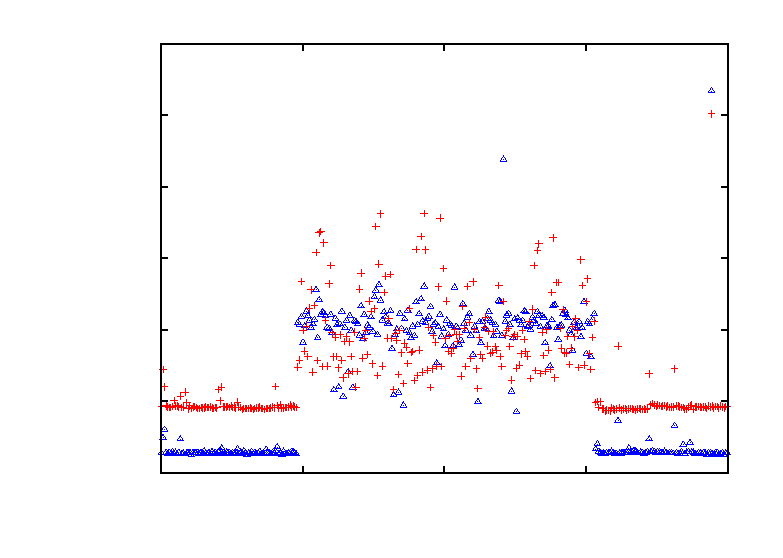
\includegraphics{fig/rtaiStress}}%
    \gplfronttext
  \end{picture}%
\endgroup
}}}%
   \hspace{14pt}%
  \subfloat[][Xenomai]{%
    \label{fig:xenoStress}%
    {\scalebox{1}{\input{fig/xenoStress}}}}%
%   \hspace{14pt}%
%   \subfloat[][M�dia sobre 50 eventos, freq��ncia de $1000 Hz$.]{%
%     \label{fig:xenoF1}%
%     {\scalebox{0.6}{\input{fig/xenoF1}}}}%
  \caption[Lat�ncia de escalonamento e de execu��o de RTAI e Xenomai]{Lat�ncia de
    escalonamento e tempo de execu��es do Kernel Linux 2.6.19.7, com RTAI e com
    Xenomai. As figuras \subref{fig:rtaiStress} e \subref{fig:xenoStress}
    representam detalhes das figuras \ref{fig:rtai}\subref{fig:rtai2} e
    \ref{fig:xeno}\subref{fig:xeno1}.}
  \label{fig:stress}%
\end{figure}







\begin{comment}



A interpreta��o proposta aqui para os resultados relativos ao estresse UDP � a
seguinte.  Quando a placa de rede recebe um pacote Ethernet, ela gera uma
interrup��o para informar o processador. Este eventualmente executa o tratador
associado a esta interrup��o. Mas, se um novo pacote cheguar antes do fim da sua
execu��o, o tratador poderia ser preemptado por uma outra execu��o dele mesmo.  Para
prevenir esta eventualidade, foi visto na se��o \label{sec:interrupt} que o \kernell
padr�o desabilita as interrup��es durante a execu��o de um tratador de
interrup��o. Al�m disso, durante a execu��o do tratador, quando o \kernell percebe
que v�rios pacotes est�o esperando na mem�ria tamp�o da placa, uma otimiza��o da
camada de rede permite que estes v�rios pacotes sejam recebidos, sem esperar novas
interrup��es. Estas opera��es acumuladas podem explicar que as interrup��es sejam
desabilitadas para tempos mais longo que o tempo de recep��o de um pacote s�.

\begin{figure}[!hbt]
  %\hfill
  %\vspace{0.2in}
  \begin{minipage}[!t]{\textwidth}
    \begin{center}  
      \centerline{\resizebox{0.8\linewidth}{!}{\input{fig/irqKern}}}
      \caption{Lat�ncia de interrup��o do \kernell Linux}
      \label{fig:irqKern}
    \end{center}
  \end{minipage}
  %\hfill
  \\
  \vspace{.4in}
  \begin{minipage}[!t]{\textwidth}
    \begin{center}  
      \centerline{\resizebox{0.8\linewidth}{!}{\input{fig/irqKernMean}}}
      \caption{Lat�ncia de interrup��o do \kernell Linux (m�dia sobre 10 valores)}
      \label{fig:irqKernMean}
    \end{center}
  \end{minipage}
  %\hfill
\end{figure}

\begin{figure}[!hbt]
  %\hfill
  %\vspace{0.2in}
  \begin{minipage}[!t]{\textwidth}
    \begin{center}  
      \centerline{\resizebox{0.8\linewidth}{!}{\input{fig/irqXeno}}}
      \caption{Lat�ncia de interrup��o do Xenomai}
      \label{fig:irqXeno}
    \end{center}
  \end{minipage}
  %\hfill
  \\
  \vspace{.4in}
  \begin{minipage}[!t]{\textwidth}
    \begin{center}  
      \centerline{\resizebox{0.8\linewidth}{!}{\input{fig/irqXenoMean}}}
      \caption{Lat�ncia de interrup��o do Xenomai (m�dia sobre 10 valores)}
      \label{fig:irqXenoMean}
    \end{center}
  \end{minipage}
  %\hfill
\end{figure}

\begin{figure}[hbt]
  \index{fig!irqXeno}
  \centering
  \input{fig/irqXeno}
  \caption{Lat�ncia de interrup��o do Xenomai}
  \label{fig:irqXeno}
\end{figure}

\begin{figure}[hbt]
  \index{fig!irqXenoMean}
  \centering
  \input{fig/irqXenoMean}
  \caption{Lat�ncia de interrup��o do Xenomai  (m�dia sobre 10 valores)}
  \label{fig:irqXenoMean}
\end{figure}

\begin{figure}[hbt]
  \index{fig!irqRTAI}
  \centering
  \input{fig/irqRTAI}
  \caption{Lat�ncia de interrup��o do RTAI}
  \label{fig:irqRTAI}
\end{figure}




  \begin{figure}
    \begin{center}
      \input{fig/realSemStr}
    \end{center}
  \end{figure}

  \begin{figure}
    \begin{center}
      % GNUPLOT: LaTeX picture with Postscript
\begingroup
  \makeatletter
  \providecommand\color[2][]{%
    \GenericError{(gnuplot) \space\space\space\@spaces}{%
      Package color not loaded in conjunction with
      terminal option `colourtext'%
    }{See the gnuplot documentation for explanation.%
    }{Either use 'blacktext' in gnuplot or load the package
      color.sty in LaTeX.}%
    \renewcommand\color[2][]{}%
  }%
  \providecommand\includegraphics[2][]{%
    \GenericError{(gnuplot) \space\space\space\@spaces}{%
      Package graphicx or graphics not loaded%
    }{See the gnuplot documentation for explanation.%
    }{The gnuplot epslatex terminal needs graphicx.sty or graphics.sty.}%
    \renewcommand\includegraphics[2][]{}%
  }%
  \providecommand\rotatebox[2]{#2}%
  \@ifundefined{ifGPcolor}{%
    \newif\ifGPcolor
    \GPcolorfalse
  }{}%
  \@ifundefined{ifGPblacktext}{%
    \newif\ifGPblacktext
    \GPblacktextfalse
  }{}%
  % define a \g@addto@macro without @ in the name:
  \let\gplgaddtomacro\g@addto@macro
  % define empty templates for all commands taking text:
  \gdef\gplbacktext{}%
  \gdef\gplfronttext{}%
  \makeatother
  \ifGPblacktext
    % no textcolor at all
    \def\colorrgb#1{}%
    \def\colorgray#1{}%
  \else
    % gray or color?
    \ifGPcolor
      \def\colorrgb#1{\color[rgb]{#1}}%
      \def\colorgray#1{\color[gray]{#1}}%
      \expandafter\def\csname LTw\endcsname{\color{white}}%
      \expandafter\def\csname LTb\endcsname{\color{black}}%
      \expandafter\def\csname LTa\endcsname{\color{black}}%
      \expandafter\def\csname LT0\endcsname{\color[rgb]{1,0,0}}%
      \expandafter\def\csname LT1\endcsname{\color[rgb]{0,1,0}}%
      \expandafter\def\csname LT2\endcsname{\color[rgb]{0,0,1}}%
      \expandafter\def\csname LT3\endcsname{\color[rgb]{1,0,1}}%
      \expandafter\def\csname LT4\endcsname{\color[rgb]{0,1,1}}%
      \expandafter\def\csname LT5\endcsname{\color[rgb]{1,1,0}}%
      \expandafter\def\csname LT6\endcsname{\color[rgb]{0,0,0}}%
      \expandafter\def\csname LT7\endcsname{\color[rgb]{1,0.3,0}}%
      \expandafter\def\csname LT8\endcsname{\color[rgb]{0.5,0.5,0.5}}%
    \else
      % gray
      \def\colorrgb#1{\color{black}}%
      \def\colorgray#1{\color[gray]{#1}}%
      \expandafter\def\csname LTw\endcsname{\color{white}}%
      \expandafter\def\csname LTb\endcsname{\color{black}}%
      \expandafter\def\csname LTa\endcsname{\color{black}}%
      \expandafter\def\csname LT0\endcsname{\color{black}}%
      \expandafter\def\csname LT1\endcsname{\color{black}}%
      \expandafter\def\csname LT2\endcsname{\color{black}}%
      \expandafter\def\csname LT3\endcsname{\color{black}}%
      \expandafter\def\csname LT4\endcsname{\color{black}}%
      \expandafter\def\csname LT5\endcsname{\color{black}}%
      \expandafter\def\csname LT6\endcsname{\color{black}}%
      \expandafter\def\csname LT7\endcsname{\color{black}}%
      \expandafter\def\csname LT8\endcsname{\color{black}}%
    \fi
  \fi
  \setlength{\unitlength}{0.0500bp}%
  \begin{picture}(7200.00,5040.00)%
    \gplgaddtomacro\gplbacktext{%
      \csname LTb\endcsname%
      \put(1254,660){\makebox(0,0)[r]{\strut{}$-1.0$}}%
      \put(1254,1125){\makebox(0,0)[r]{\strut{}$0.0$}}%
      \put(1254,1590){\makebox(0,0)[r]{\strut{}$1.0$}}%
      \put(1254,2055){\makebox(0,0)[r]{\strut{}$2.0$}}%
      \put(1254,2520){\makebox(0,0)[r]{\strut{}$3.0$}}%
      \put(1254,2985){\makebox(0,0)[r]{\strut{}$4.0$}}%
      \put(1254,3450){\makebox(0,0)[r]{\strut{}$5.0$}}%
      \put(1254,3915){\makebox(0,0)[r]{\strut{}$6.0$}}%
      \put(1254,4380){\makebox(0,0)[r]{\strut{}$7.0$}}%
      \put(1386,440){\makebox(0,0){\strut{}$ 0$}}%
      \put(2163,440){\makebox(0,0){\strut{}$ 10$}}%
      \put(2940,440){\makebox(0,0){\strut{}$ 20$}}%
      \put(3717,440){\makebox(0,0){\strut{}$ 30$}}%
      \put(4495,440){\makebox(0,0){\strut{}$ 40$}}%
      \put(5272,440){\makebox(0,0){\strut{}$ 50$}}%
      \put(6049,440){\makebox(0,0){\strut{}$ 60$}}%
      \put(6826,440){\makebox(0,0){\strut{}$ 70$}}%
      \put(220,2520){\rotatebox{90}{\makebox(0,0){\strut{}Lat\^encia em $\mu s$}}}%
      \put(4106,110){\makebox(0,0){\strut{}Tempo de execu\c{c}\~ao em $s$}}%
      \put(4106,4710){\makebox(0,0){\strut{}Xenomai sem estresse, com ajusto - Lat\^encia de escalonamento}}%
    }%
    \gplgaddtomacro\gplfronttext{%
    }%
    \gplbacktext
    \put(0,0){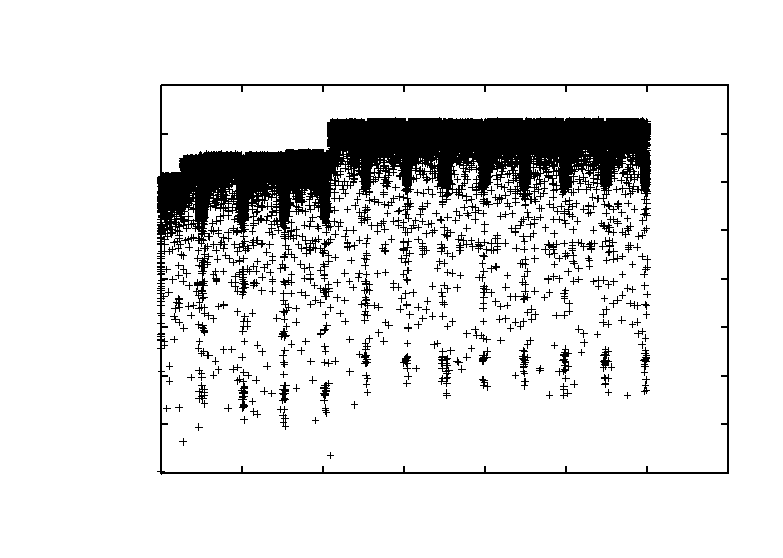
\includegraphics{fig/diffSemStr}}%
    \gplfronttext
  \end{picture}%
\endgroup

    \end{center}
  \end{figure}


  \begin{figure}
    \begin{center}
      % GNUPLOT: LaTeX picture with Postscript
\begingroup
  \makeatletter
  \providecommand\color[2][]{%
    \GenericError{(gnuplot) \space\space\space\@spaces}{%
      Package color not loaded in conjunction with
      terminal option `colourtext'%
    }{See the gnuplot documentation for explanation.%
    }{Either use 'blacktext' in gnuplot or load the package
      color.sty in LaTeX.}%
    \renewcommand\color[2][]{}%
  }%
  \providecommand\includegraphics[2][]{%
    \GenericError{(gnuplot) \space\space\space\@spaces}{%
      Package graphicx or graphics not loaded%
    }{See the gnuplot documentation for explanation.%
    }{The gnuplot epslatex terminal needs graphicx.sty or graphics.sty.}%
    \renewcommand\includegraphics[2][]{}%
  }%
  \providecommand\rotatebox[2]{#2}%
  \@ifundefined{ifGPcolor}{%
    \newif\ifGPcolor
    \GPcolorfalse
  }{}%
  \@ifundefined{ifGPblacktext}{%
    \newif\ifGPblacktext
    \GPblacktextfalse
  }{}%
  % define a \g@addto@macro without @ in the name:
  \let\gplgaddtomacro\g@addto@macro
  % define empty templates for all commands taking text:
  \gdef\gplbacktext{}%
  \gdef\gplfronttext{}%
  \makeatother
  \ifGPblacktext
    % no textcolor at all
    \def\colorrgb#1{}%
    \def\colorgray#1{}%
  \else
    % gray or color?
    \ifGPcolor
      \def\colorrgb#1{\color[rgb]{#1}}%
      \def\colorgray#1{\color[gray]{#1}}%
      \expandafter\def\csname LTw\endcsname{\color{white}}%
      \expandafter\def\csname LTb\endcsname{\color{black}}%
      \expandafter\def\csname LTa\endcsname{\color{black}}%
      \expandafter\def\csname LT0\endcsname{\color[rgb]{1,0,0}}%
      \expandafter\def\csname LT1\endcsname{\color[rgb]{0,1,0}}%
      \expandafter\def\csname LT2\endcsname{\color[rgb]{0,0,1}}%
      \expandafter\def\csname LT3\endcsname{\color[rgb]{1,0,1}}%
      \expandafter\def\csname LT4\endcsname{\color[rgb]{0,1,1}}%
      \expandafter\def\csname LT5\endcsname{\color[rgb]{1,1,0}}%
      \expandafter\def\csname LT6\endcsname{\color[rgb]{0,0,0}}%
      \expandafter\def\csname LT7\endcsname{\color[rgb]{1,0.3,0}}%
      \expandafter\def\csname LT8\endcsname{\color[rgb]{0.5,0.5,0.5}}%
    \else
      % gray
      \def\colorrgb#1{\color{black}}%
      \def\colorgray#1{\color[gray]{#1}}%
      \expandafter\def\csname LTw\endcsname{\color{white}}%
      \expandafter\def\csname LTb\endcsname{\color{black}}%
      \expandafter\def\csname LTa\endcsname{\color{black}}%
      \expandafter\def\csname LT0\endcsname{\color{black}}%
      \expandafter\def\csname LT1\endcsname{\color{black}}%
      \expandafter\def\csname LT2\endcsname{\color{black}}%
      \expandafter\def\csname LT3\endcsname{\color{black}}%
      \expandafter\def\csname LT4\endcsname{\color{black}}%
      \expandafter\def\csname LT5\endcsname{\color{black}}%
      \expandafter\def\csname LT6\endcsname{\color{black}}%
      \expandafter\def\csname LT7\endcsname{\color{black}}%
      \expandafter\def\csname LT8\endcsname{\color{black}}%
    \fi
  \fi
  \setlength{\unitlength}{0.0500bp}%
  \begin{picture}(7200.00,5040.00)%
    \gplgaddtomacro\gplbacktext{%
      \csname LTb\endcsname%
      \put(1386,660){\makebox(0,0)[r]{\strut{}$292.0$}}%
      \put(1386,1125){\makebox(0,0)[r]{\strut{}$294.0$}}%
      \put(1386,1590){\makebox(0,0)[r]{\strut{}$296.0$}}%
      \put(1386,2055){\makebox(0,0)[r]{\strut{}$298.0$}}%
      \put(1386,2520){\makebox(0,0)[r]{\strut{}$300.0$}}%
      \put(1386,2985){\makebox(0,0)[r]{\strut{}$302.0$}}%
      \put(1386,3450){\makebox(0,0)[r]{\strut{}$304.0$}}%
      \put(1386,3915){\makebox(0,0)[r]{\strut{}$306.0$}}%
      \put(1386,4380){\makebox(0,0)[r]{\strut{}$308.0$}}%
      \put(1518,440){\makebox(0,0){\strut{}$ 0$}}%
      \put(2276,440){\makebox(0,0){\strut{}$ 10$}}%
      \put(3035,440){\makebox(0,0){\strut{}$ 20$}}%
      \put(3793,440){\makebox(0,0){\strut{}$ 30$}}%
      \put(4551,440){\makebox(0,0){\strut{}$ 40$}}%
      \put(5309,440){\makebox(0,0){\strut{}$ 50$}}%
      \put(6068,440){\makebox(0,0){\strut{}$ 60$}}%
      \put(6826,440){\makebox(0,0){\strut{}$ 70$}}%
      \put(220,2520){\rotatebox{90}{\makebox(0,0){\strut{}Lat\^encia em $\mu s$}}}%
      \put(4172,110){\makebox(0,0){\strut{}Tempo de execu\c{c}\~ao em $s$}}%
      \put(4172,4710){\makebox(0,0){\strut{}Xenomai com estresse, com ajusto - Lat\^encia de escalonamento}}%
    }%
    \gplgaddtomacro\gplfronttext{%
    }%
    \gplbacktext
    \put(0,0){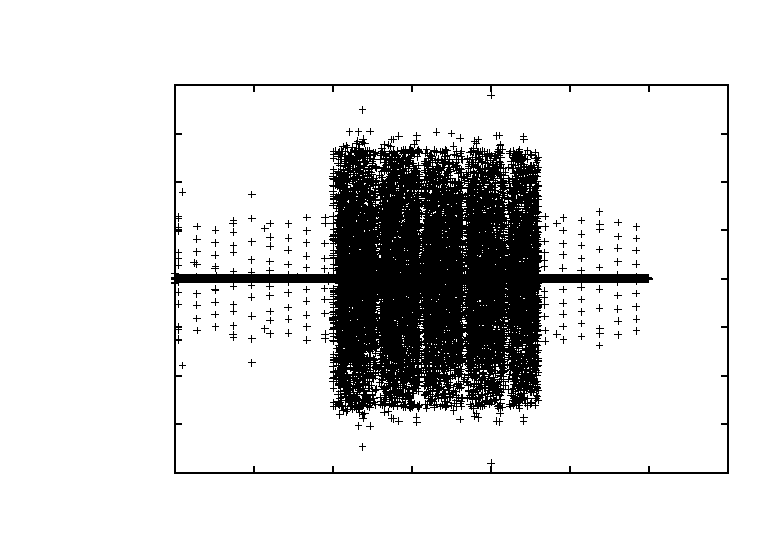
\includegraphics{fig/realComStr}}%
    \gplfronttext
  \end{picture}%
\endgroup

    \end{center}
  \end{figure}

  \begin{figure}
    \begin{center}
      \input{fig/diffComStr}
    \end{center}
  \end{figure}

\end{comment}


\chapter{Conclus�o}
\label{sec:conclusao}

Nesta disserta��o, foi descrito um novo protocolo baseado em dois an�is l�gicos que
organiza a coexist�ncia de comunica��es com requisitos temporais cr�ticos e
n�o-cr�ticos, num mesmo barramento Ethernet.

Gra�as � utiliza��o da abordagem TDMA para estruturar o anel cr�tico, \doris{}
garante previsibilidade para as aplica��es com requisitos temporais cr�ticos,
enquanto a utiliza��o da abordagem com bast�o circulante impl�cito serviu para
controlar eficientemente o acesso ao meio referente ao anel n�o-cr�tico.  Esta
combina��o permitiu garantir, por um lado, a confiabilidade do protocolo pelo
isolamento temporal dos dois modos de comunica��o e, por outro, otimizar o uso
da banda.

O protocolo \doris{} foi especificado formalmente em TLA+ (\ing{Temporal Logic of
  Actions}) e v�rias propriedades temporais do protocolo foram verificadas pelo
verificador de modelos TLC (\ing{Temporal Logic Checker}). Especificar o protocolo
em TLA+ permitiu adquirir uma compreens�o precisa do sistema e das suas
funcionalidades, antes de partir para a fase de implementa��o. Esta fase se
beneficiou da especifica��o formal, que foi utilizada como base para o trabalho de
codifica��o. Apesar de a escolha de usar uma plataforma j� existente ter
impossibilitado, em parte, um melhor aproveitamento da especifica��o, pois a
codifica��o do protocolo teve que seguir o padr�o da plataforma, chegou-se �
conclus�o que a fase de especifica��o facilitou v�rias decis�es importantes
tomadas durante a fase de implementa��o do protocolo.

Para o desenvolvimento deste projeto, uma plataforma de Tempo Real baseada no
Sistema Operacional de Prop�sito Geral - Linux foi escolhida.  As principais
motiva��es para tal escolha foram a boa divulga��o deste sistema de c�digo aberto
nas comunidades de pesquisa e a exist�ncia de extens�es de tempo real para
Linux. Algumas destas extens�es foram apresentadas e experimentos foram realizados
para medir as lat�ncias de interrup��o e ativa��o de tarefas de tempo real.  Os
resultados obtidos permitiram confirmar a viabilidade do uso destes ambientes
operacionais para desenvolver \doris. Em particular, as plataformas de c�digo aberto
RTAI e Xenomai / Linux apresentaram propriedades temporais satisfat�rias,
conseguindo garantir o escalonamento de tarefas de tempo real com tempos de
lat�ncias abaixo de 20 microsegundos.

A implementa��o de \doriss foi ent�o realizada na plataforma Xenomai / Linux,
podendo ser facilmente transportada para a plataforma RTAI / Linux.  A pilha de rede
determinista RTnet, j� desenvolvida para estas duas plataformas, foi aproveitada, e
\doriss foi inserido, sob a forma de uma nova disciplina desta pilha.  Devido �
complexidade do desenvolvimento de um protocolo de rede determinista num ambiente
operacional tal como Xenomai / Linux, a implementa��o foi limitada a uma vers�o
simplificada de \doris, sem o mecanismo de reserva. No entanto, um mecanismo 
de configura��o din�mica do anel n�o-cr�tico foi desenvolvido para diminuir a
sobrecarga gerada pela transmiss�o de mensagens de controle.

O prot�tipo de \doris, com sua estrutura operacional em dois an�is, foi utilizado
para realizar alguns experimentos que confirmaram a capacidade do protocolo \doriss
 atender requisitos de sistemas h�bridos, compostos de aplica��es com requisitos
temporais cr�ticos e n�o-cr�ticos. Em particular, os experimentos mostraram que
\doriss consegue garantir determinismo para as mensagens cr�ticas e taxas de
transmiss�es altas para a comunica��o n�o-cr�tica. Os mesmos experimentos realizados
com a pilha RTnet, sem disciplina de acesso ao meio, provocaram desvios significativos
nos tempos de recep��o das mensagens cr�ticas e perdas de mensagens n�o-cr�ticas.

No decorrer deste trabalho, v�rios aspectos foram abordados de maneira superficial. Outros
foram deixados para trabalhos futuros dado o horizonte temporal para concluir a presente
disserta��o. Trabalhos futuros poder�o: 

\begin{itemize}
\item Completar o estudo experimental do comportamento de \doriss com cen�rios de 
  comunica��o de redes industriais. Em particular, cen�rios de falhas dever�o ser utilizados
  para testar as propriedades de confiabilidade de \doris.
\item Estudar os protocolos de gerenciamento da composi��o e reconfigura��o din�mica
  dos grupos, e propor solu��es adequadas para aumentar a confiabilidade e a
  flexibilidade de \doris{}.
\item Acrescentar a implementa��o de \doriss com o mecanismo de reserva descrito na
  sua especifica��o.
\item Definir pol�ticas de escalonamento das mensagens, baseadas no mecanismo de
  reserva e em poss�veis extens�es deste mecanismo. O aumento do n�mero de
  \ing{slots} de reserva por \ing{chip} poder�, por exemplo, ser utilizado para
  aumentar a flexibilidade do protocolo.
\end{itemize}

Finalmente, por ser um protocolo distribu�do, descentralizado e determinista,
baseado num �nico barramento compartilhado, com capacidades de toler�ncia a falhas
de omiss�o de mensagens e de paradas de esta��es, \doriss apresenta caracter�sticas
interessantes para ser adaptado no contexto de redes sem fios. No entanto, tal
aplica��o depende da implementa��o de um protocolo eficiente de gerenciamento e
reconfigura��o din�mica da composi��o dos an�is cr�ticos e n�o-cr�ticos.

Acredita-se que este trabalho tenha trazido contribui��es para o campo
de pesquisa de redes para sistemas de tempo real. Alguns conceitos aqui
apresentados, como o mecanismo de reserva e a ado��o de m�todos formais na fase
inicial de concep��o do protocolo de comunica��o, dever�o certamente influenciar
trabalhos de pesquisa futuros nesta �rea.

% \include{capitulo8}
% ...
% \include{capituloN}
%
% Importante: Use \xchapter ao inves de \chapter, conforme exemplo abaixo.

%%
%% Parte pos-textual
%%
\backmatter

% Apendices
% Comente se n??o houver ap??ndices
\appendix

% Eh aconselhavel criar cada apendice em um arquivo separado, digamos
% "apendice1.tex", "apendice.tex", ... "apendiceM.tex" e depois
% inclui--los com:
% \include{apendice1}
% \include{apendice2}
% ...
% \include{apendiceM}

% Bibliografia
% ?? aconselh??vel utilizar o BibTeX a partir de um arquivo, digamos "biblio.bib".
% Para ajuda na cria????o do arquivo .bib e utiliza????o do BibTeX, recorra ao
% BibTeXpress em www.cin.ufpe.br/~paguso/bibtexpress
\bibliographystyle{abntex2-alf}
\bibliography{biblio}

% Colofon
% Inclui uma pequena nota com referencia a UFPEThesis
% Comente para omitir
%\colophon

%% Fim do documento
\end{document}
